\hypertarget{element_8h}{
\section{src/element.h File Reference}
\label{element_8h}\index{src/element.h@{src/element.h}}
}
Facet planar geometry for graphical representation purposes. 

{\tt \#include $<$vector$>$}\par


Include dependency graph for element.h:\nopagebreak
\begin{figure}[H]
\begin{center}
\leavevmode
\includegraphics[width=65pt]{element_8h__incl}
\end{center}
\end{figure}


This graph shows which files directly or indirectly include this file:\nopagebreak
\begin{figure}[H]
\begin{center}
\leavevmode
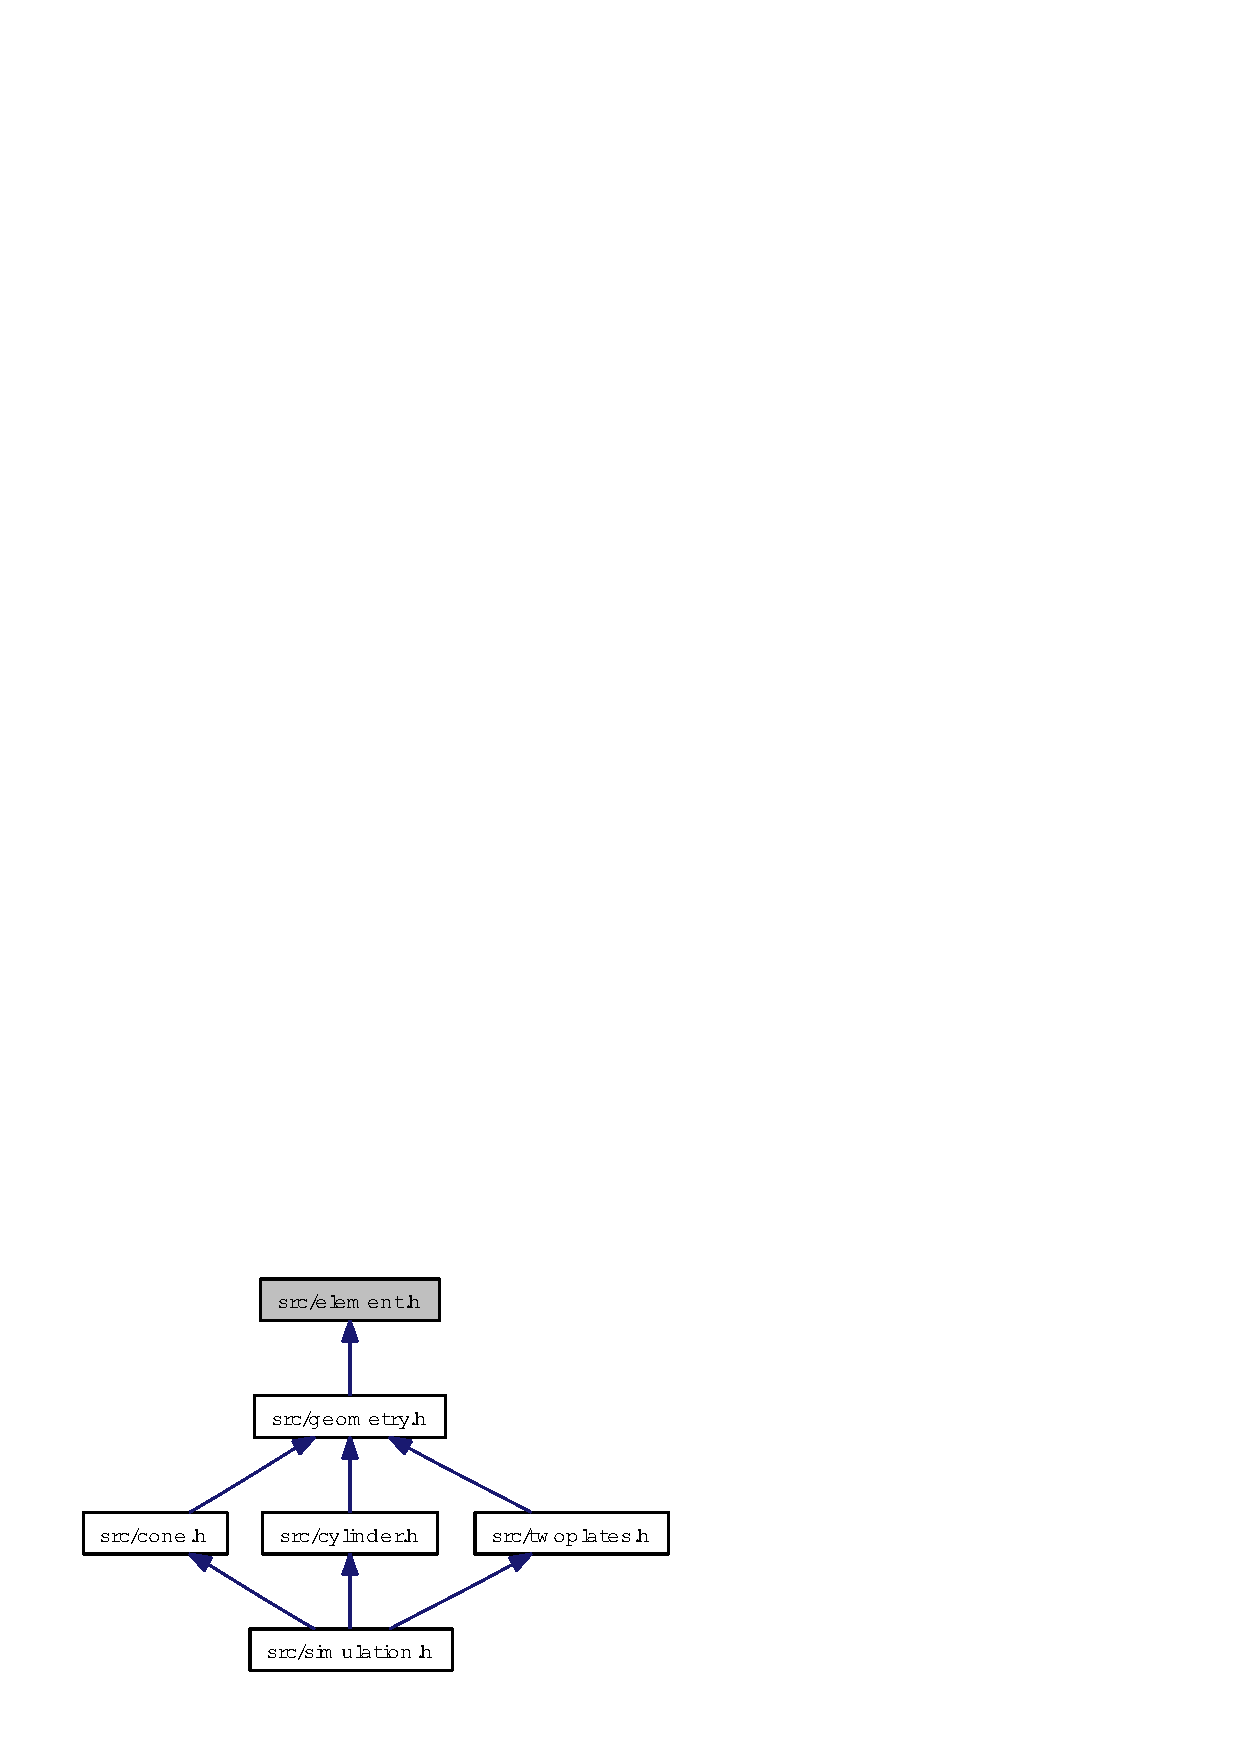
\includegraphics[width=162pt]{element_8h__dep__incl}
\end{center}
\end{figure}
\subsection*{Classes}
\begin{CompactItemize}
\item 
class \hyperlink{classElement}{Element}
\end{CompactItemize}


\subsection{Detailed Description}
Facet planar geometry for graphical representation purposes. 

Uses the \hyperlink{classNode}{Node} class for the defining the vertices. Usually, the dimensions are proportional to the number of sections (longitudinal) and sectors (transversal divisions).

\begin{Desc}
\item[Author:]Daniel Iglesias $<$\href{mailto:daniel.iglesias@ciemat.es}{\tt daniel.iglesias@ciemat.es}$>$ \end{Desc}
